\documentclass[preprint,12pt]{elsarticle}

\usepackage{amsmath,amssymb,amsfonts}
\usepackage{graphicx}
\usepackage{booktabs}
\usepackage{hyperref}
\usepackage{cleveref}
\usepackage{xcolor}
\usepackage{bm}
\usepackage{enumitem}

% math_commands.tex — shared notation for DSC CMB paper
\newcommand{\R}{\mathbb{R}}
\newcommand{\Z}{\mathbb{Z}}
\newcommand{\N}{\mathbb{N}}
\newcommand{\calL}{\mathcal{L}}
\newcommand{\calM}{\mathcal{M}}

% DSC-specific
\newcommand{\lnln}{\ln^2}
\newcommand{\ac}{a_c}
\newcommand{\kopt}{k_{\mathrm{opt}}}
\newcommand{\mudyn}{\mu_{\mathrm{dyna}}}
\newcommand{\ceff}{c^2_{\mathrm{eff}}}
\newcommand{\Hinfty}{H_\infty}
\newcommand{\tP}{t_{\mathrm{P}}}
\newcommand{\lP}{\ell_{\mathrm{P}}}
\newcommand{\nside}{N_{\mathrm{side}}}

% Operators
\DeclareMathOperator*{\argmin}{arg\,min}
\DeclareMathOperator{\Tr}{Tr}


\graphicspath{{../figures/}}

% Supplementary numbering: S1, S2, ... and Fig. S1, ...
\renewcommand{\thesection}{S\arabic{section}}
\renewcommand{\thefigure}{S\arabic{figure}}
\renewcommand{\thetable}{S\arabic{table}}
\renewcommand{\theequation}{S\arabic{equation}}

\journal{Next Research}

\begin{document}

\begin{frontmatter}
\title{Supplementary Material:\\
Differentiable Discrete Symplectic Cosmology: Cross-Scale Empirical Tests of a $1/\ln^2(t)$ Cooling Law}
\author[hust]{Liang Wang}
\ead{wangliang.f@gmail.com}
\address[hust]{School of Artificial Intelligence and Automation, Huazhong University of Science and Technology, 430070, P.R. China}
\end{frontmatter}

This Supplementary Material collects (i) the per-pillar figures for the Block~2
Hubble-parameter tests whose headline statistics are tabulated in the main text
(\cref{sec:sm_block2}), and (ii) the full report of the Block~3 CMB lattice
forward model and differentiable inverse reconstruction (\cref{sec:sm_cmb}),
which is methodological rather than empirical. Section, figure, table, and
equation numbers are prefixed ``S'' throughout. References to the main-text
pillars (A--O) use the same labels as the main manuscript.

\section{Block 2 per-pillar figures}
\label{sec:sm_block2}

This section reproduces the individual figures for Pillars~B, D, E, F, G, H,
and~J, summarized in Table~2 of the main text. The accompanying numbers and
interpretation are given in the main text; here we provide the full plots.

\paragraph{Pillar B: King 2012 295-absorber three-model fit.}
The full King \emph{et al.}~(2012) catalog gives reduced $\chi^2 = 0.881$ for the
DSC $p=2$ model vs.\ $0.878$ for the constant null ($\Delta\chi^2 \approx 0$,
$\Delta\mathrm{BIC} = +5.7$ favoring the null); the joint quasar + atomic-clock
bound is $|\Gamma| < 0.30$ (\cref{fig:sm_king2012}).

\begin{figure}[htbp]
  \centering
  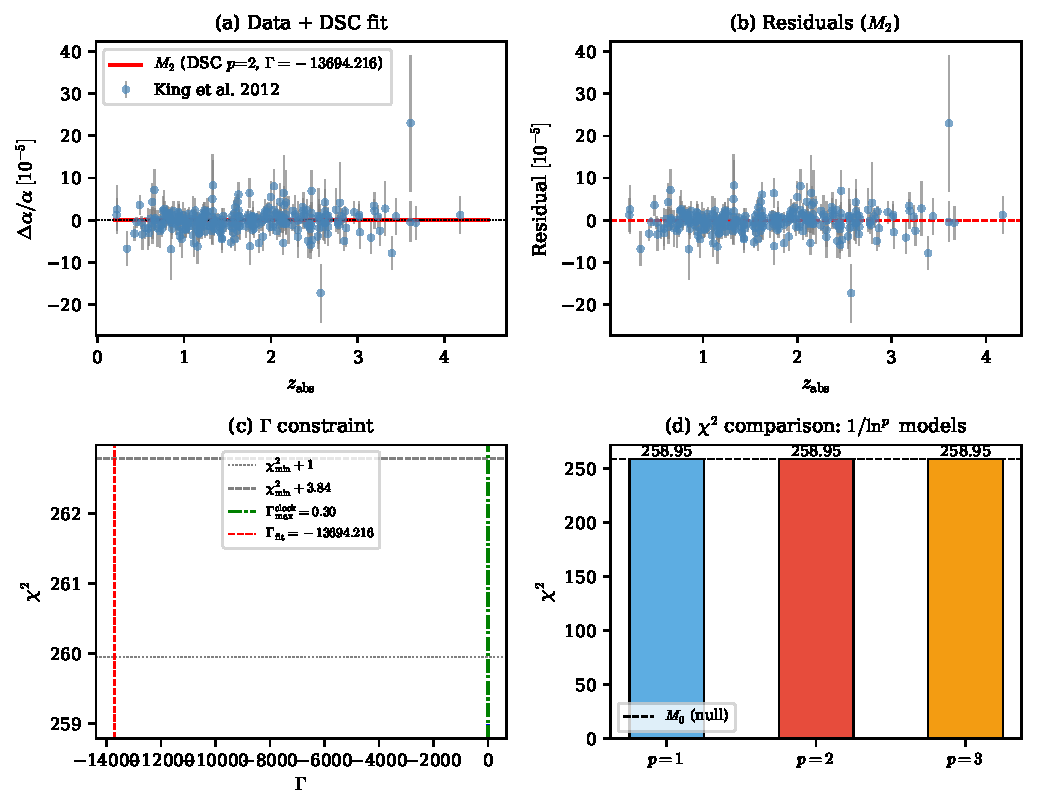
\includegraphics[width=\columnwidth]{fig20_quasar_293_fit.pdf}
  \caption{Three-model comparison on the full King \emph{et al.}~(2012) 295-absorber sample.
  Top: data with best-fit DSC $p = 2$ curve and constant null.
  Bottom: $\chi^2(\Gamma)$ profile and joint clock + quasar bound $|\Gamma| < 0.30$.
  $\Delta {\rm BIC}({\rm DSC}, {\rm null}) = +5.7$ favors the null.}
  \label{fig:sm_king2012}
\end{figure}

\paragraph{Pillar K (cont.): cut-by-cut sensitivity of the King 2012 catalog.}
The Keck-only subset ($N = 141$) yields $\Gamma = +6.4 \pm 1.9$ ($3.3\sigma$),
the VLT-only subset ($N = 154$) yields $\Gamma = -2.0 \pm 1.1$ ($1.8\sigma$,
opposite direction), and 200 random 128-absorber subsamples give a median
$\Delta\chi^2 = 0.4$ (16--84\% interval $[0.04, 1.27]$), none reaching $31.5$
(\cref{fig:sm_pillar_K}).

\begin{figure}[htbp]
  \centering
  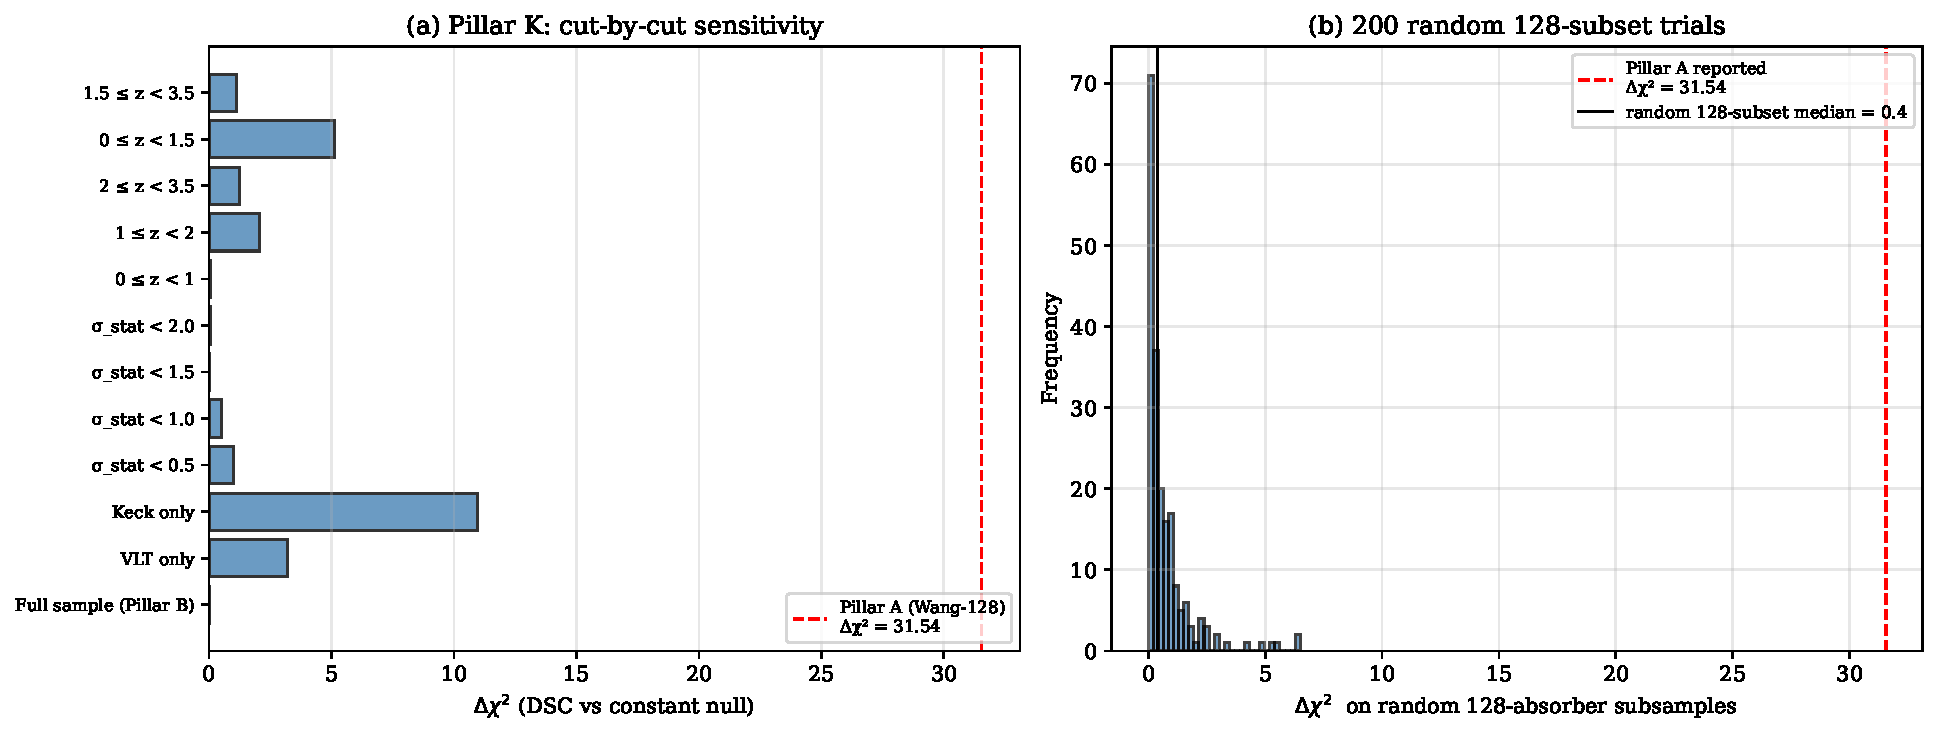
\includegraphics[width=\columnwidth]{fig27_pillar_K_subset.pdf}
  \caption{Pillar~K (King 2012 subset scan): (a) cut-by-cut $\Delta\chi^2$ vs the constant null; the Keck-only subset gives $\Delta\chi^2 = 11.0$, while the VLT-only subset gives $\Gamma$ of opposite sign.
  (b) 200 random 128-absorber subsamples give a median $\Delta\chi^2 = 0.4$; the headline value $31.5$ is not reproduced by any random cut.}
  \label{fig:sm_pillar_K}
\end{figure}

\paragraph{Pillar D: CAMB + BAO Fisher constraint.}
The combined Fisher matrix gives $\sigma(\gamma_{\rm eff}) \sim 1.2 \times 10^4$,
leaving the DSC dark-energy correction unconstrained at present sensitivity; the
maximum fractional change to the TT spectrum is $\sim 12.5\%$ at the largest
scales (\cref{fig:sm_camb_fisher}).

\begin{figure}[htbp]
  \centering
  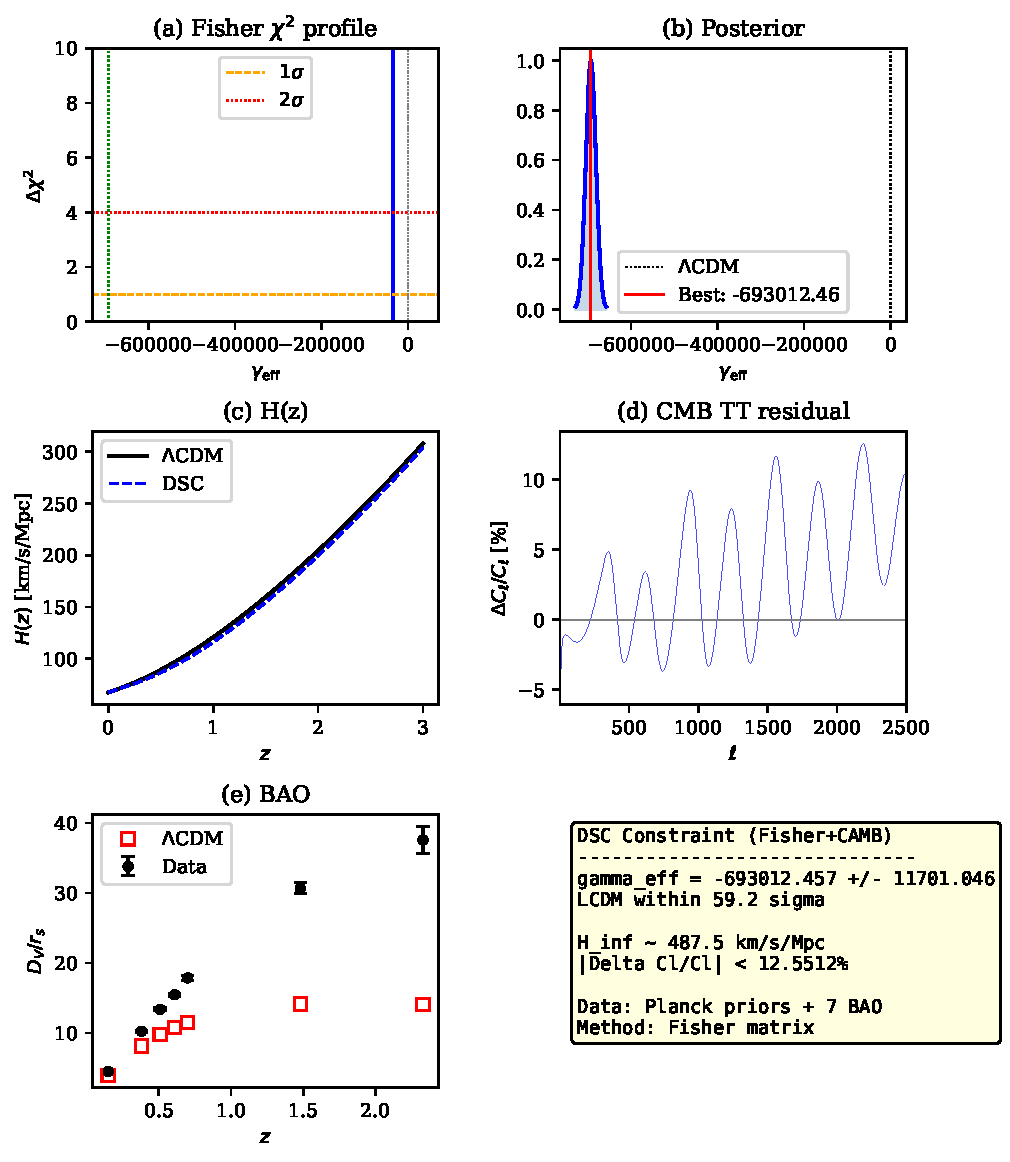
\includegraphics[width=\columnwidth]{fig21_camb_fisher.pdf}
  \caption{CAMB-based Fisher constraint on the DSC effective dark-energy parameter $\gamma_{\rm eff}$.
  Top: $\Lambda$CDM-vs-DSC TT power spectrum residual at $\gamma_{\rm eff} = 1$.
  Bottom: BAO $D_V/r_d$ derivatives over $z \in [0.15, 2.33]$.
  Combined Fisher gives $\sigma(\gamma_{\rm eff}) \sim 1.2 \times 10^4$.}
  \label{fig:sm_camb_fisher}
\end{figure}

\paragraph{Pillar E: late-time perturbation stability.}
All five stability criteria (C1: $H^2 > 0$; C2: $\dot H < 0$; C3: monotone growth
$D(a)$; C4: $c_s^2 = 0$; C5: $\Lambda$CDM-consistent $w_{\rm eff}(z=0)$) pass over
$a \in [10^{-10}, 1]$ and $\gamma_{\rm eff} \in [0, 10]$ (\cref{fig:sm_late_stability}).

\begin{figure}[htbp]
  \centering
  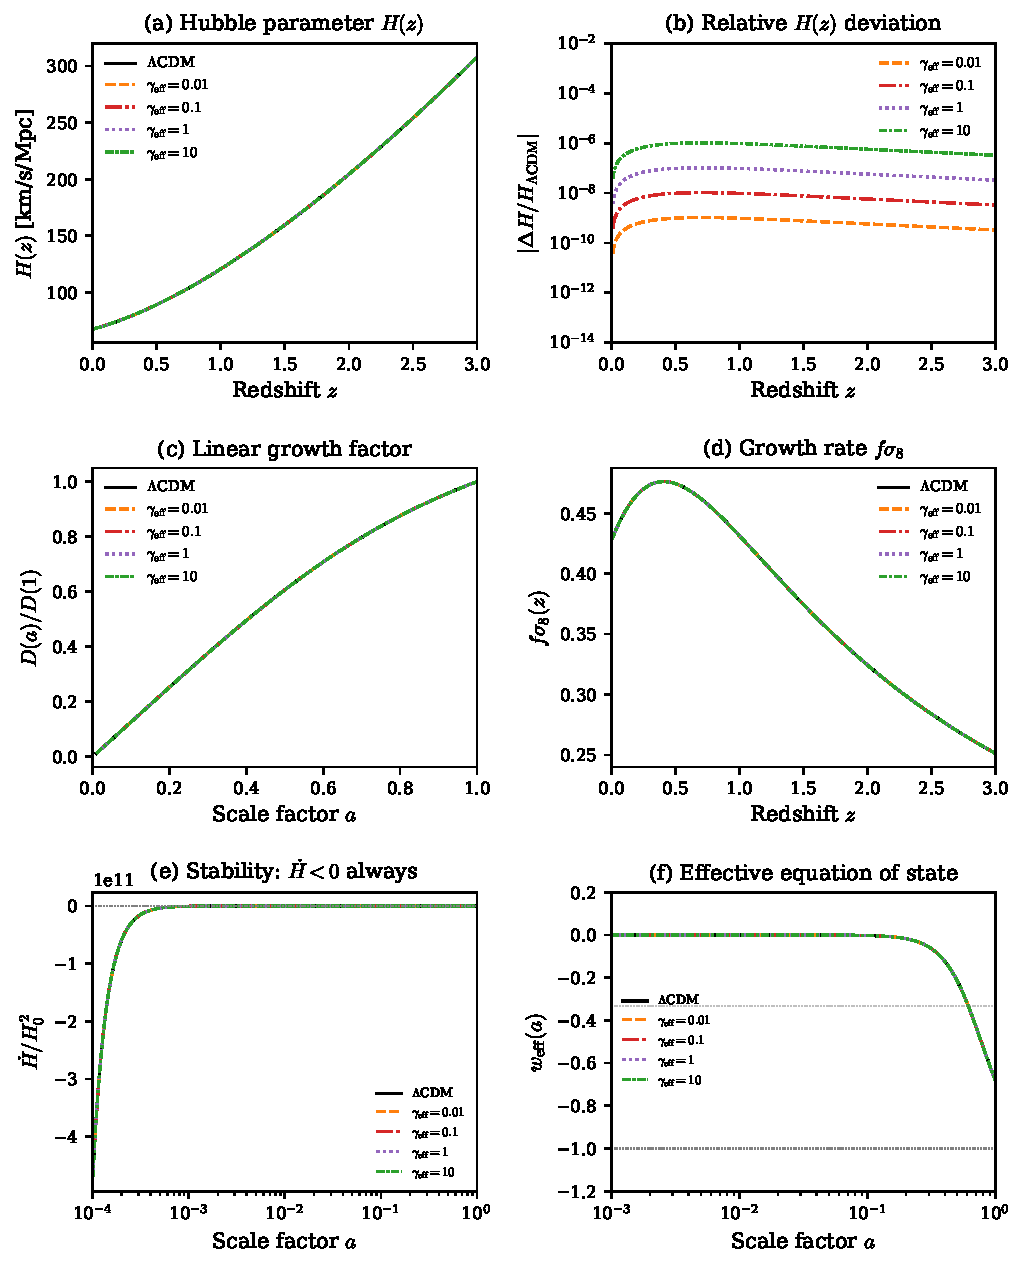
\includegraphics[width=\columnwidth]{fig22_late_stability.pdf}
  \caption{Late-time stability scan for the DSC $\Lambda(t)$.
  All five stability criteria (C1--C5) pass over $a \in [10^{-10}, 1]$ and $\gamma_{\rm eff} \in [0, 10]$.}
  \label{fig:sm_late_stability}
\end{figure}

\paragraph{Pillar F: cosmic chronometer $H(z)$.}
$\Lambda$CDM gives $\chi^2/{\rm dof} = 0.49$; DSC gives $4.01$ and is degenerate
with constant $H_0$ over $z \in [0.07, 1.97]$ (\cref{fig:sm_cc}), because $\xi(z)$
varies by only $\Delta\xi \approx 0.11$ across this band vs.\ $0.86$ at anchor
scale (Pillar~M).

\begin{figure}[htbp]
  \centering
  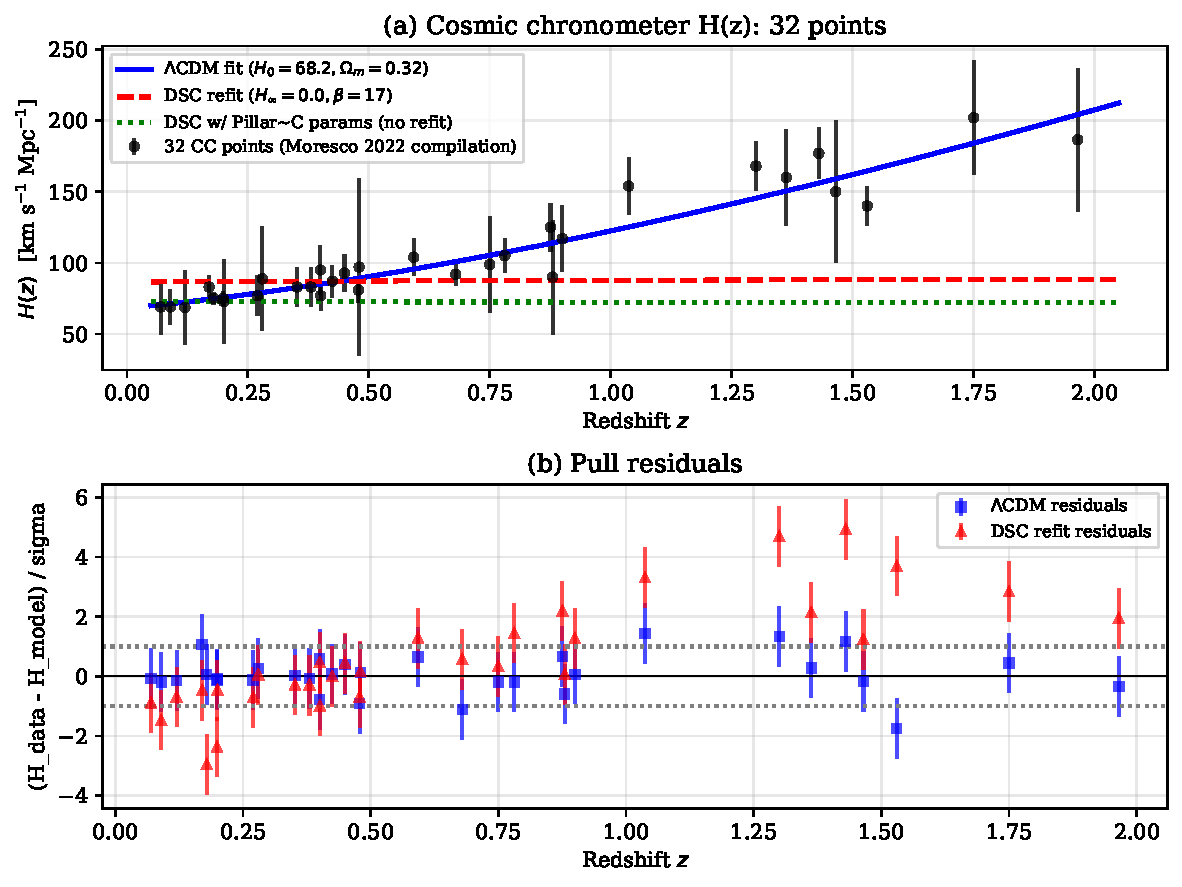
\includegraphics[width=\columnwidth]{fig23_cc_hz_pillar_F.pdf}
  \caption{Pillar~F: cosmic chronometer $H(z)$.
  $\Lambda$CDM ($\chi^2/{\rm dof} = 0.49$) describes the data; the DSC ansatz ($\chi^2/{\rm dof} = 4.01$) is degenerate with constant $H_0$ over $z \in [0.07, 1.97]$.}
  \label{fig:sm_cc}
\end{figure}

\paragraph{Pillar G: Pantheon+ Type Ia supernovae.}
The 1580-SN Pantheon+ sample with full covariance gives $\Lambda$CDM
$\chi^2/{\rm dof} = 0.88$ and DSC $1.27$ ($\Delta\chi^2 = +617$, $\sim 25\sigma$
preference for $\Lambda$CDM; \cref{fig:sm_pantheon}).

\begin{figure}[htbp]
  \centering
  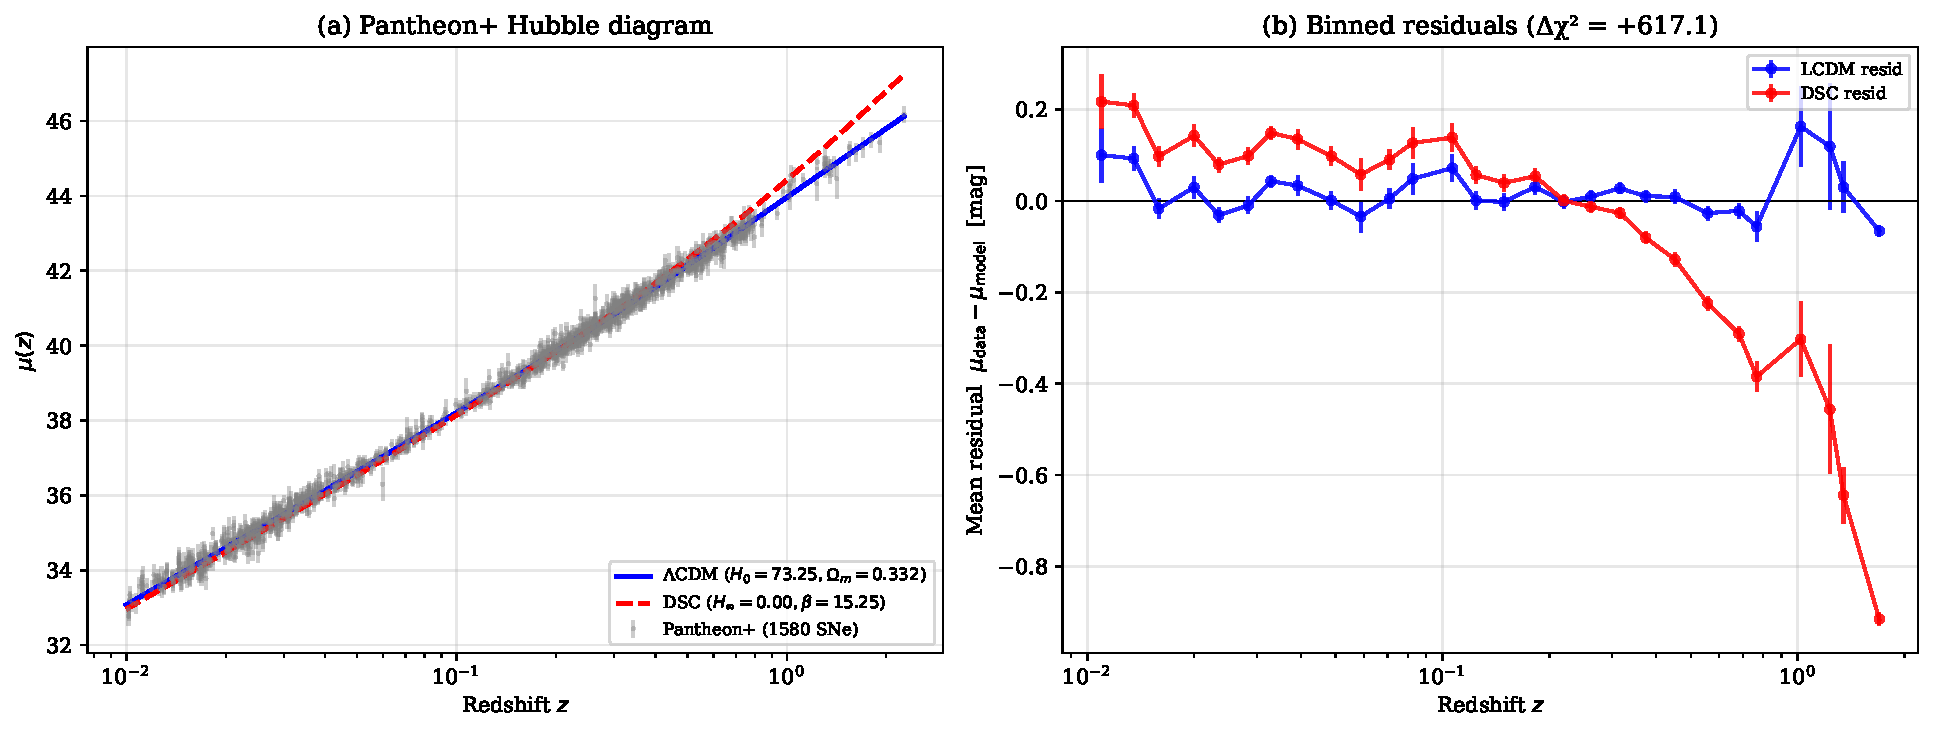
\includegraphics[width=\columnwidth]{fig24_pantheon_pillar_G.pdf}
  \caption{Pillar~G: Pantheon+ Hubble diagram and binned residuals.
  $\Lambda$CDM achieves $\chi^2/{\rm dof} = 0.88$, DSC achieves $1.27$ ($\Delta\chi^2 = +617$).}
  \label{fig:sm_pantheon}
\end{figure}

\paragraph{Pillar H: DESI DR2 BAO.}
$\Lambda$CDM gives $\chi^2/{\rm dof} = 1.07$, CPL $1.16$, DSC $\chi^2 = 14036$
(catastrophic): DSC predicts approximately constant $D_M/r_d$ and $D_H/r_d$,
contrary to the observed monotone trends (\cref{fig:sm_desi}).

\begin{figure}[htbp]
  \centering
  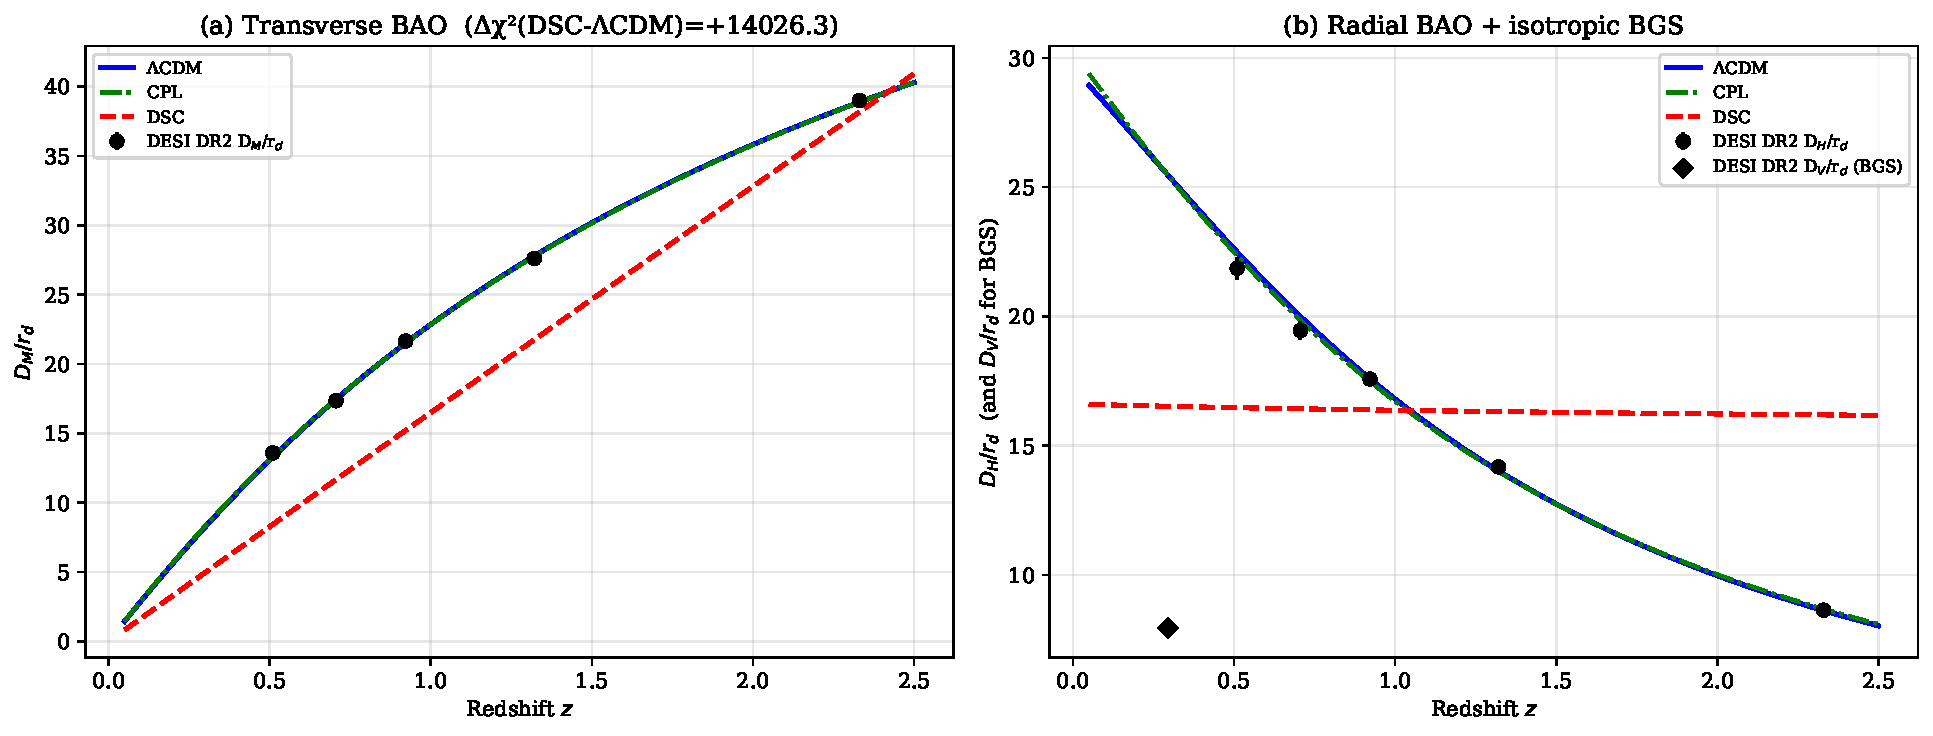
\includegraphics[width=\columnwidth]{fig25_desi_pillar_H.pdf}
  \caption{Pillar~H: DESI DR2 BAO. $\Lambda$CDM ($\chi^2/{\rm dof}=1.07$) and CPL ($\chi^2/{\rm dof}=1.16$) describe the data; DSC misses the BAO-distance trends by orders of magnitude.}
  \label{fig:sm_desi}
\end{figure}

\paragraph{Pillar J: joint 1623-constraint dataset.}
Combining DESI + Pantheon$+$ + cosmic chronometers, $\Lambda$CDM gives
$\chi^2/{\rm dof} = 0.96$; CPL ($w_0w_a$) gives $0.95$ and is mildly preferred
($\Delta {\rm BIC} = -2.6$); DSC gives $23.7$ ($\Delta\chi^2 = +36{,}878$ vs.\
$\Lambda$CDM; \cref{fig:sm_pillar_J}).

\begin{figure}[htbp]
  \centering
  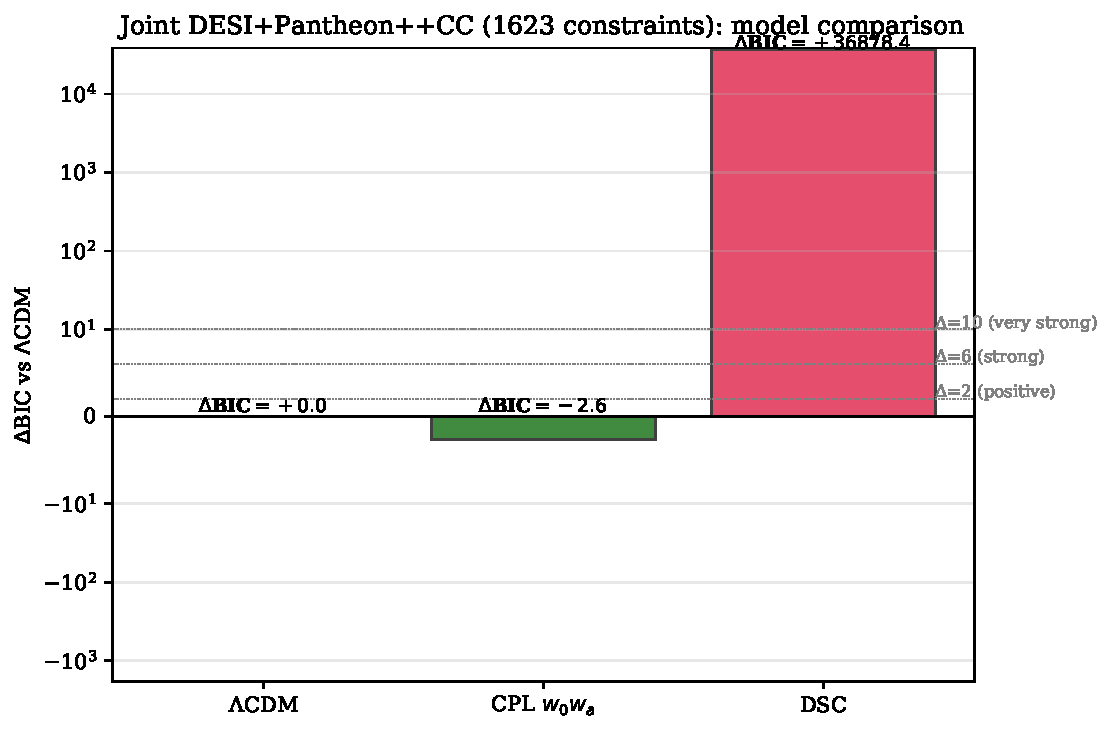
\includegraphics[width=0.8\columnwidth]{fig26_pillar_J_joint.pdf}
  \caption{Pillar~J: joint $\Delta {\rm BIC}$ vs $\Lambda$CDM on 1623 late-time constraints.
  CPL is mildly preferred ($\Delta {\rm BIC} = -2.6$); the simple DSC ansatz is ruled out at $\Delta {\rm BIC} \sim 4\times 10^4$.}
  \label{fig:sm_pillar_J}
\end{figure}

\input{sections/S_cmb_lattice}

\bibliographystyle{elsarticle-num}
\bibliography{references}

\end{document}
